% !TeX program = lualatex

\documentclass[a4paper]{article}
\usepackage[scale=0.7]{geometry}
\usepackage[french]{babel}
\usepackage{multicol}
\usepackage{graphicx}
\usepackage{fontspec}
\defaultfontfeatures{Mapping=tex-text}

\author{Suvam Battacharya, Jean Carpentier, Yu Jia Cheong,\\
Léo Gaspard, Damien Ménigaux et Hua Ting Yao\\
Tutorés par Karim El Alami, Cyril Colin et Steve Oudot\\
Coordonnés par Frank Nielsen}
\title{Gestion intelligente de l'électricité d'un bâtiment par prédiction de la
demande énergétique}
\date{22 avril 2016}

\begin{document}

\maketitle
\clearpage

\renewcommand{\abstractname}{Préambule}
\begin{abstract}
\addcontentsline{toc}{section}{Préambule}

Fugiat est voluptatum et odio. Harum enim sed quo. Et possimus harum sit.

In quisquam voluptatem nemo ut accusantium libero minima adipisci. Enim
    occaecati molestiae porro dignissimos molestiae. Ut eum autem repellat
    reprehenderit doloribus dolorem totam amet. Et error consequuntur voluptatem
    et illum.

Facilis explicabo ipsam asperiores qui dolores soluta sit unde. Corrupti
    blanditiis minus enim nesciunt libero. Ex cumque in alias nostrum ut
    veritatis commodi. Error voluptates neque in aut. Perspiciatis corporis
    voluptas odio dolorem quaerat. Facere odio cupiditate explicabo voluptatem
    asperiores eum dolor.

Explicabo aperiam exercitationem aut quia quisquam ut. Non laborum dolores
    aliquid rem ab voluptatem quos. Eos quibusdam culpa veniam. Facere eum in
    optio. Aperiam culpa quos perspiciatis facilis aliquid autem libero.

Ut et reprehenderit voluptas consequatur eum magnam. Debitis eos accusantium
    assumenda. Voluptates tempore et ratione accusamus deserunt consequatur
    animi eius. Beatae et qui cupiditate impedit ullam. Facilis quis officia
    magnam.

\end{abstract}
\clearpage

\tableofcontents
\clearpage
\addcontentsline{toc}{section}{Introduction}
\section{Optimisation de la consommation énergétique à l’aide de l’analyse de données : dernières tendances}


\begin{multicols}{2}
\subsection{Contexte général de l'étude}
Depuis quelques années, les techniques d’apprentissage automatique - ou Machine Learning, et d’analyse de données se sont largement répandues, dans des domaines variés : de l’économie à la physque, de la prise de décision dans le milieu de l’entreprise aux voitures automatiques. Les applications sont mutliples. Mais l’un des domaines les plus prometteurs dans lesquels l’analyse de données peut se réveler révolutionnaire est l’optimisation de la consommation énergétique. Puisque la demande énergétique de nos sociétés s’est considérablement accrue dans les dernières décennies, le carctère crucial d’une telle optimisation s’est affirmée avec encore plus de force. Cela explique la profusion des travaux scientifiques dans ce champs, d’autant plus que la "data science" est prometteuse aussi bien par ses perspectives économiques que par son efficacité face aux prolèmes d’optimisation actuels.

\subsection{Recueillir les données}
L’analyse de données nous fournit un regard nouveau sur nos consommations énergétiques domestique et industrielle. Les avancées techonologiques en matière de mesures ont tout particulièrment facilité la collection de données sur des durées étendues. On pourrait citer les interval meters data pour illustrer ce propos.

\subsection{L’entreprise}

Les entreprises s’intéressant à ce domaine sont de plus en plus nombreuses. Depuis 2010, FirstFuel a conduit des milliers de ces analyses. IBM a lancé le software IBM TRIRIGA Energy Optimization destiné à réduire la consommation de certaines organisations en les accompagnant depuis le lancement. Une autre enreprise, Stem Inc., utilise du big data, des analyses prédictives, du cloud computing et du stockage d’énergie pour réduire l’amplitude des pics de consommation, réduire les factures électriques et supprimer la dépendance aux nouvelles industries.
Locas, une entreprise spécialisée dans les logiciels d’analyse de données, se consacre à employer ses talents pour trouver de nouvelles méthodes d’optimisation énergétique, particulièrement à l’aide de panneaux photovoltaïque. Elle a aussi développé un moteur de prédiction couplé à son produit Virtual Irradiance, qui sépare une image envoyée par un satellite en quatre signaux reconnus par le software comme quatre imageries différentes (la couverture nuageuse, les turbulences atmosphériques...). Ce moteur met ensuite en oeuvre ses algorithmes pour calculer son régime d’utilisation optimal à n’importe quel moment ultérieur.

\subsection{Théories}

Les problèmes de régression linéaire et de classification sont communs en matière de rentabilité énergétique. Par exemple, la régression est utile lorsqu’on cherche à prédire la demande totale d’énergie d’un bâtiment entier dans l’heure en prenant en input la situation météorologique et d’autres données concernant l’utilisation de son espace intérieur. Ce genre de régression fait naître des perspectives d’amélioration en prenant en compte des paramètres mieux choisis, afin d’allonger la validité des prédicitons sur plusieurs heures. Les données de consommation énergétique soulèvent une kyrielle de problèmes de supervised et unsupervised learning. Ceux ci regroupent aussi bien du clustering, de la recherche d’anomalie ou des time series. Ainsi, pour un batiment donné, il est possible de rechercher des constructions "similaires" dans une base de données construite avec l’expérience. On s’attend à ce que ceux là aient une utilisation énergétique similaire. Ceci est un exemple de problème faisant appel au semi-supervised learning et de clustering. Mais la technique du Time series est employée encore plus communément en matière d’utilisation de l’énergie; deux exemples sont le monitoring and verifying (M\&V) et la prédiction des pics de demande. Monitoring signifiant les méthodes pour prévoir les demandes énergétiques d’un bâtiment précis dans des circonstances inhabituelles. Verifying (ou quantifying) les méthodes utiles afin de veiller à l’étendue de l’économie lors de réaménagement techniques ou de changements de stratégies opérationnelles. La valeur des charges liées à la demande sur une facture d’électricité est fondée sur la plus forte capacité réclamée par l’utilisateurs. Ainsi, prédire les pics de demande permet de prendre des mesures visant à lisser la consommation, et minimiser la demande en énergie durant une période donnée. De plus, chaque bâtiment est tôt ou tard soumis à des changements majeurs de configuration, tels qu’un résident déménageant, ou bien des anomalies comme le  dysfonctionnement d’un équipement. Ces changement doivent être pris en considération par les méthodes mentionnées ci-dessus.

\subsection{Challenges}
D’autres problèmes sont aussi communs qu’inévitables : des valeurs manquantes, des bruits dans les données. Mais contrairement à ce qu’on pourrait penser, recueillir des données fidèles n’est pas le plus grand défi des analystes. Ceux-ci, lorsqu’on leur demande de citer leur plus gros obstacles, ne mentionnent la qualité des données ou leur fidélité que dans un cas sur cinq. Parmis les barrières commerciales et industrielles contre lesquelles se heurtent les entreprises employant ces méthodes, la plupart sont culturelles ou de l’ordre de la gestion pure (marketing envers les propriété privées...) plutôt que d’être liées aux données ou à la technologie. Le plus gros frein à leur diffusion est le côté novateur donc inconnu et le manque de compréhension du caractère bénéifque de celles-ci sur "les affaires". Pour les propriétés privées, le défi s’illustre par la rentabilité de la méthode sur le long-terme uniquement, alors que son implémentation s’accompagne de frais d’installation, alors que le marketing dans ce domaine lui fait encore défaut. Mais la Data Science recèle un énorme potentiel. Une étude de Ventana Research indique que seuls 12\% des manufactures employant l’analyse des données a atteint une "maturité" complète dans cette utilisation.
\end{multicols}

\clearpage

\section{Enjeux et motivations}
\begin{multicols}{2}
\subsection{Réduire la facture énergétique}
Notre Projet Scientifique Collectif s’inscrit dans la perspective du développement d’une startup dédiée à l’optimisation de la consommation électrique : eLum. Nous avons accompagné la mise en place des algorithmes servant à contrôler un système électrique composé de panneaux solaires, batteries et d’un circuit consommateur (ici, une usine). L’objectif était d’isoler intégralement ce système du reste du réseau.
Le projet que nous avons mis en oeuvre repose sur des caractéristiques intrinsèques à l’énergie électrique :
— le prix de l’électricité est variable au cours de la journée ;
— le rapport des prix est de 1,6 entre le prix de jour et celui de nuit pour une petite usine consommant de 3 à 36 kWh ;
— la production électrique d’un système de panneaux solaires est variable au cours de la journée et ne peut pas toujours couvrir les besoins instantanés de l’usine ; et
— la consommation électrique d’une usine est similaire d’une journée à l’autre et peu sujette à des variations aléatoires de grande ampleur.

\subsection{Utiliser une batterie pour optimiser les prix de l’électricité}
Actuellement, il est seulement possible d'optimiser de façon limitée ces caractéristiques en consommant en priorité l’électricité solaire quand celle du réseau est plus chère et inversement. Nous ajoutons donc au problème une batterie dont le but est grossièrement de stocker l’énergie la nuit pour une utilisation ultérieure en journée. La production d’électricité à base de panneaux solaire est variable, nous utilisons donc le principe suivant :
— cas où la production dépasse la consommation : stocker cette énergie gratuite dans la batterie ; et
— cas où la production est inférieure à la consommation : puiser dans les réserves de la batterie.
Remarque : dans le cadre de notre Projet Scientifique Collectif, on suppose qu’il est économiquement préférable d’éviter l’utilisation de l’électricité issue du réseau. Le détail de l’étude financière du coût de la batterie, des différences tarifaires entre heures pleines et heures creuses n’est donc pas menée.

\subsection{Prédire la consommation et la production électrique}
La prédiction du niveau de la batterie à avoir au début de la journée de deux facteurs inconnus : la consommation et la production énergétiques sur la journée à venir.
Par exemple, si la journée qui vient est très ensoleillée, le surplus de production électrique suffira à combler les besoins pour la fin de la journée, quand les panneaux ne produisent plus. Il n’est donc pas nécessaire d’utiliser le réseau électrique pour recharger la batterie pendant la nuit. A l’inverse, si la journée est prévue nuageuse, la production des panneaux solaires sera faible et ne pourra pas suffisamment recharger la batterie pour assurer le fonctionnement en fin de journée. Il faut donc charger la batterie au préalable.
Notre objectif a donc été de créer un ensemble d’algorithmes d’apprentissage automatique (machine learning) pour prédire la consommation et la production électrique. Il se sert des données collectées par des capteurs installés au sein d’une usine marocaine par eLum. Il a fallu en premier lieu déterminer les facteurs (features) dont dépend la consommation energétique. Ensuite il a fallu s’intéresser aux facteurs, principalement météorologiques, qui influencent la production des panneaux solaires.
La valeur ajoutée de notre travail provient de notre désir de construire une prédiction adaptative, dans le sens ou les algorithmes sont implémentés au sein d'un programme perpétuellement relancé. Cela permet, si la prédiction diverge par rapport aux valeurs relevées par les capteurs des panneaux et du réseau, de la relancer en modifiant les paramètres des modèles.
Guidés par ces réflexions, on a pu construire des prédictions robustes et intelligentes. On a tenu à développer des algorithmes de prédiction à court terme, plus fidèles sur le moment, et à long terme, plus justes sur la journée, afin de garantir l'adaptabilité du résultat.


\end{multicols}

\clearpage

\addcontentsline{toc}{section}{L'étude}
\section{Objectifs et composantes}
\begin{multicols}{2}
\subsection{Une prédiction de la consommation intelligente}
Le signal à prédire fournit par les capteurs possède des caractéristiques de périodicité typiques d'une consommation industrielle. En voici un tracé sur 11 jours.

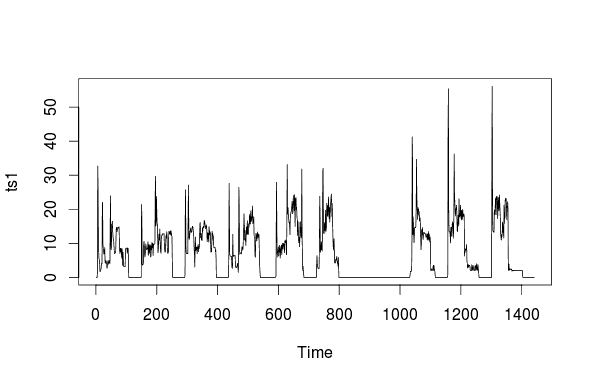
\includegraphics[width=0.45\textwidth]{./images/traceconsom.png}

La nuit, la consommation est nulle, ainsi que pendant les vacances, les weeks ends, mais pas toujours. Les heures d'ouvertures des machines sont relativement peu variables. Certaines semaines sont plus chargées que d'autres. Certains jours sont nettement moins chargés que le reste de la semaine. Parfois, les machines restent allumées la nuit. Il s'agit donc d'une production assez régulière pour être prédite, mais qui demande naturellement des précautions.
L'approche adoptée est l'analyse de time series. On ne cherche pas à lier ce signal à d'autres grandeurs. La prédiction fera éventuellement appel à du machine learning, mais seulement avec des features artificielles élaborées au préalable, et non observées.
Le désir de la start up Elum est davoir une bonne prédiction sur 24h.

\subsection{Une prédiction de la production des panneaux solaires}


Et aspernatur porro quis earum quia temporibus non corrupti. Omnis dolorum
    deleniti eos nulla. Rerum eaque aut adipisci ducimus enim.

Et mollitia voluptas expedita eum veniam repellat consectetur. Dicta nihil
    temporibus est. Odit et sed temporibus officia ratione nulla labore magnam.
    At tenetur aspernatur quod itaque quia aperiam. Explicabo nostrum soluta
    ducimus commodi.

Autem non officiis qui quos sit expedita labore ut. Quia voluptas et quo sequi
nihil vel et. Quisquam explicabo quod rerum dolore. Doloremque reprehenderit non
non sed consequatur autem. Dolores perferendis quidem vel adipisci quia quasi.

Veniam aliquam voluptatem molestiae ullam. Modi veniam sunt explicabo voluptate
minima laudantium esse vel. Adipisci qui culpa amet sint non dolore tempore
voluptate.

Et aspernatur porro quis earum quia temporibus non corrupti. Omnis dolorum
    deleniti eos nulla. Rerum eaque aut adipisci ducimus enim.

Et mollitia voluptas expedita eum veniam repellat consectetur. Dicta nihil
    temporibus est. Odit et sed temporibus officia ratione nulla labore magnam.
    At tenetur aspernatur quod itaque quia aperiam. Explicabo nostrum soluta
    ducimus commodi.



\end{multicols}

\clearpage

\section{Prédiction de la production}

\begin{multicols}{2}

\subsection{Démarche et méthodologie}
\subsubsection{Sélection des features}
Un étude est fait d’abord des correlation des variables dans les données de SIRTA avec la puissance produite par les panneaux photovoltaique. 


\begin{tabular}{l c r}
  Facteur & Correlation \\
  Measured Solar Irradiance & 0.978788 \\
  Temperature dans l’air & 0.394982 \\
  Wind Speed & 0.133656 \\
  Wind Direction & -0.049585 \\
  Solar Zenith Angle & -0.667123 \\
  Solar Azimuth Angle & 0.040420 \\
\end{tabular}
\tablename{ Correlation avec P1(W)}

Parmi les variables météos, l’irradiance a un correlation le plus marqué, et donc la suite de la prédiction est basé pour la plupart sur l’irradiance.

\subsubsection{Preprocessing de données}

Les données datetime sont d'abord linearisés dans un séries de 1 et 0 pour les mois, jours, heures, et minutes. 

Trois algorithmes principales étaient utilisés ensuite pour apprendre à prédire les données : Support Vector Machine (SVM), Random Forest, et Neural Networks.

Ces trois algorithmes sont ensuite evalué avec un fonctionne d'erreur quadratique, qui prend pour chaque instant, la différence entre la valeur vraie et la valeur predictée, divisée par la valeur vraie à cette instante. 

\subsection{Développement théorique}
\subsubsection{Support Vector Machines (SVM)}

Support Vector Machine  est une méthode d’apprentisage supervisé, qui utilise des fonctions noyaux pour classifier ou pour régresser les données. L’algorithme fait ensuite une optimisation basé sur le produit scalaire des points dans un espace de grande dimension nommé le « feature space ». Ceci est défini selon la fonction noyau donnée. SVM est souvent utiliser dans les cas où les dimensions des données sont plus grandes que le nombre des données. Bien que ceci ne soit pas le cas pour la prévision de la production, le choix d’utiliser SVM dans la prévision vient de la possibilité de customisation les noyaux permettant un contrôle plus fine du problème. 

Des apprentissages étaient faits avec un noyau linéaire, un noyau polynomial, et un noyau Radial Basis Function (RBF). Les résultats sont les suivants et la décision était ensuite prise de continuer avec le noyau RBF. 

Linear R$^{2} $score : 0.958624795379

RBF R$^{2}$ score : 0.96155168192

Polynomial R$^{2}$ score : 0.553626719589

L'algorithme RBF a deux paramètres intrinsèques au problème, C et gamma. C permets un contrôle du lissage de la frontière de la décision, tandis que gamma contrôle l’influence d’un donnée individu. 

Un tuning des paramètres montre que la configuration des paramètres optimales pour la situation, sont gamma = 0.2 et C = 36. La démarche est expliqué en détail dans l'annexe. 

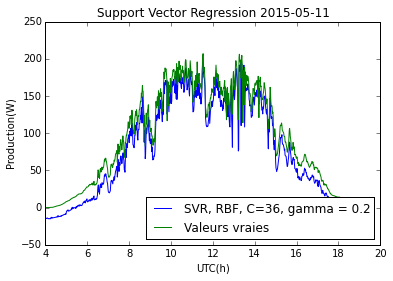
\includegraphics[width=0.45\textwidth]{./images/11maysvm.png}

Le temps pris pour le tuning de SVM à cette configuration était dans les environs de 45 minutes, avec les erreurs suivants : 

Quadratique erreur relative : 32.83

R2 Score : 0.9675

Racine carré de RMS : 12.822

\subsubsection{Random Forest}
Un étape additionel de pre-processing était fait avec l'algorithme Random Forest. Le choix de ne pas utiliser ce variable en plus pour le SVM était fait en vue du temps d'apprentisage lent pour le SVM. 

Les journées sont d’abord catégorisées dans plusieurs types selon les fluctuations des données, d’un moment à la prochaine, c’est à dire, comment une fonction est lisse. Pour cela, deux fonctions sont définies : MaxStep et VarStep. MaxStep calculent la maximum différence entre deux données consécutive d’une journée, VarStep la variance des différences entre deux données consécutive d’une journée. Ensuite, en appliquant un algorithme de K-Means, les jours sont catégorisées dans 3 groupes. On varie à la fin le nombre des clusters selon la performance du code suivant.


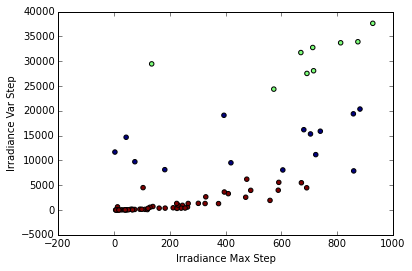
\includegraphics[width=0.45\textwidth]{./images/categoriesgraph.png}


Les groupements des données est donc ajoutés et considérés comme une variable additionnelle. 




\subsubsection{Neural Network}
Ea quia aut officiis ipsa ab suscipit quidem. Consequuntur inventore aliquam
    exercitationem eligendi sit. Explicabo doloremque aut dolores distinctio
    commodi voluptatem iure. Praesentium iusto sed quia sed. Quae nulla unde et
    qui animi culpa. Deleniti laudantium ea quia rerum laudantium placeat rem.

Dolor tempore minima asperiores ratione laborum architecto. Commodi perspiciatis
    quisquam maxime quos ipsa nemo inventore. Iusto aut inventore in quod.

Dolorem et quae qui dolor dolor dolor. Atque omnis nostrum aliquid atque
    reiciendis sed voluptatibus non. Voluptatem atque pariatur possimus et quam.
    Et enim possimus soluta ratione deleniti perferendis.

Laborum quia minima modi aut sit minima saepe voluptatum. Qui dolor officia quam
    magnam velit itaque. Velit ullam qui error harum dolorem debitis.

Modi delectus eveniet saepe eum. Sit est hic id maxime corporis quasi assumenda.
    Porro eius adipisci qui repellat nisi totam molestias. Voluptatem quis
    impedit omnis sit enim autem.

Cumque ad sunt esse maiores nihil nihil esse. Eum porro quidem ut cum voluptatem
    et sequi natus. Aperiam recusandae est deserunt occaecati molestiae. Autem
    suscipit praesentium officia. Hic ipsum in culpa facilis minus quia omnis
    pariatur.

Ducimus rerum veritatis a. Voluptas qui dignissimos est consequatur deserunt
    necessitatibus ea. Placeat suscipit aut porro dolor.

Et aspernatur porro quis earum quia temporibus non corrupti. Omnis dolorum
    deleniti eos nulla. Rerum eaque aut adipisci ducimus enim.

Et mollitia voluptas expedita eum veniam repellat consectetur. Dicta nihil
    temporibus est. Odit et sed temporibus officia ratione nulla labore magnam.
    At tenetur aspernatur quod itaque quia aperiam. Explicabo nostrum soluta
    ducimus commodi.

Autem non officiis qui quos sit expedita labore ut. Quia voluptas et quo sequi
nihil vel et. Quisquam explicabo quod rerum dolore. Doloremque reprehenderit non
non sed consequatur autem. Dolores perferendis quidem vel adipisci quia quasi.

Veniam aliquam voluptatem molestiae ullam. Modi veniam sunt explicabo voluptate
minima laudantium esse vel. Adipisci qui culpa amet sint non dolore tempore
voluptate.

Ut et quae aut. Adipisci libero quasi vero dolorem maiores. Consequuntur ipsa
voluptas ut. Aperiam et magni necessitatibus tempora veniam ratione.

At et non aut tempore. Debitis et corporis quo ut. Et non assumenda sed
repellat.

Nobis sed id nemo. Impedit ab aut nostrum earum quisquam quae quis. Laudantium
dolor in reiciendis exercitationem quo molestias velit.

Quo perferendis est reprehenderit doloribus ex consequatur. Vel ut maiores
quidem quod error corporis omnis sint. Ea nemo sapiente doloremque consequatur.

Eos maiores quae corrupti quo itaque. Asperiores doloremque delectus optio
nihil. Ipsum cupiditate architecto praesentium voluptatem quod expedita tempora.
Quisquam et odit aliquid non asperiores officiis consequatur possimus.

Id minima totam sunt vel molestiae quia. Voluptatem ut unde inventore occaecati
minima assumenda. Molestiae animi explicabo facere doloremque.

Adipisci non quisquam voluptas. Explicabo quisquam itaque recusandae. Incidunt
quasi libero vel deleniti quis eius et officia. Vel harum aut sapiente officia.

Ipsum sunt libero laborum autem eligendi. Reiciendis et reiciendis occaecati qui
sit velit magni. Ab necessitatibus est illo consectetur neque iste fuga.

Omnis consequatur veniam consequuntur odio atque cum maiores molestiae. Suscipit
explicabo voluptatem voluptates dolores excepturi. Iste voluptatem omnis qui
inventore explicabo sed incidunt. Dolor autem vitae rerum vel commodi
reiciendis. Magnam quidem fuga possimus nihil reiciendis sapiente dolorum quo.
Repellendus doloremque velit non qui cum.

\end{multicols}

\subsection{Résultats}
Omnis consequatur veniam consequuntur odio atque cum maiores molestiae. Suscipit
explicabo voluptatem voluptates dolores excepturi. Iste voluptatem omnis qui
inventore explicabo sed incidunt. Dolor autem vitae rerum vel commodi
reiciendis. Magnam quidem fuga possimus nihil reiciendis sapiente dolorum quo.
Repellendus doloremque velit non qui cum.

\clearpage
\section{Prédiction de la consommation}

\begin{multicols}{2}

Libero qui magni ex dolorem quia. Quod qui corrupti voluptatum et aut.
    Laboriosam numquam pariatur est.

Inventore et amet illo perferendis eum molestiae molestias. Ut esse aut
    voluptatem consequuntur deleniti qui. Sapiente ut voluptatem consequatur
    dolores.

Praesentium voluptatum odit qui molestiae non est. Magni ipsa sunt quo esse
    dolores saepe. Omnis explicabo laborum dolorem culpa ut dolor
    necessitatibus. Quae sit commodi sapiente repellat qui. Adipisci vel
    occaecati odit dolorem doloremque officiis quisquam. Corporis non aut veniam
    architecto.

Et accusantium fuga sunt odio sunt soluta. Voluptatem reprehenderit fuga
    distinctio accusamus quo sed aut. Quod quo nam et error et labore
    voluptatem. Est iure dignissimos qui atque labore rerum. Quis recusandae et
    qui. Ad et animi mollitia fuga quia doloribus atque.

Beatae quia debitis earum sint. Molestiae aut reprehenderit minus sunt. Delectus
    culpa qui velit deserunt vero minima. Vel hic rerum eligendi. Et iusto est
    perspiciatis possimus. Aperiam laborum in est et eum nisi.

Molestias sit iure eum ad temporibus minima at. Aut officiis vitae dolor minus
    molestiae. Consectetur et id illo. At recusandae quia eos. Quaerat est iure
    et excepturi sit et et quaerat.

Asperiores non in laborum. Fugit ratione sit dolores dicta et. Corporis
    architecto error et voluptatem quis. Eius magni quas nihil eum minima
    architecto ipsam.

Et corrupti molestiae ut. Nam eius placeat assumenda aut ducimus. Magnam iusto
    est necessitatibus. Sunt qui molestiae non excepturi aperiam commodi
    debitis. Laborum placeat aliquid amet voluptatem aspernatur dicta quo. Vitae
    praesentium quidem reprehenderit sequi.

Minima impedit voluptatibus tempora exercitationem sunt qui enim. Sed sit non
    aut nihil deserunt nulla in voluptatem. Distinctio fugit quia culpa sed
    reprehenderit ut possimus laborum. Ut at harum eum harum. Qui optio cumque
    eum nam similique. Libero minus dolorum est aut deleniti eum hic.

Officia corrupti et dolorum. Nobis minima quod ut est. Eius ducimus maiores amet
    nesciunt quia harum provident sed.

Vel officiis voluptas esse eligendi hic doloremque ad. Facilis odio veritatis
    veritatis delectus eaque sed quia. Dolor libero aut qui.

Tempora voluptates ipsum aut laudantium mollitia aut ut iure. Eveniet nulla
    quaerat et inventore voluptates. Eligendi neque deleniti veritatis similique
    et. Non qui consectetur laborum repellendus ab perspiciatis.

Qui dolores rem voluptatem quod quae aspernatur doloribus. Dolorem quibusdam eos
    quibusdam incidunt et accusamus. Ipsam consequatur laborum harum odio. Et
    eos sit a et quaerat. Ad culpa dignissimos ea officia unde.

Consequatur cupiditate dolorem culpa. Aperiam adipisci molestiae voluptate optio
    animi. Beatae aspernatur ducimus omnis voluptatem sunt eaque. Accusamus
    similique nulla vel quod consequuntur.

Fugiat delectus voluptas ut quis. Quia quia aliquid voluptatum vel illo et
veritatis. Cupiditate dicta repudiandae voluptas qui quo id iure reprehenderit.
Officiis iste in ipsum corrupti sed qui. Beatae odio sed corrupti quae
doloremque iure. Quia omnis et consequatur quo cum.

Ipsum sit laboriosam dolores nostrum. Et incidunt minima reprehenderit rerum non
ut voluptas. Est quidem optio sunt culpa fugit et.

Et voluptas autem consectetur est ducimus sit quo magnam. Modi non velit
aliquam. Consequuntur eveniet qui in dignissimos molestiae aliquid id dolore.
Officia perspiciatis beatae magni est laudantium earum. Nulla voluptates sed
doloremque et earum facilis repellat inventore. Sit maxime autem commodi
voluptas.

Eum et eius vitae. Iure eius inventore omnis velit quia et. Magnam dolorem ut
quasi quas. Quidem ea est totam et vel minus. Ipsum deserunt et dolore.

Aut est inventore in quis perferendis. Dolorem voluptatibus est sit dolorum odit
doloremque. Itaque error dolores qui fugit praesentium sunt. Ipsam consequatur
dolor nihil omnis error et. Similique in animi quidem quam sed ratione non
animi.

Adipisci vitae ab exercitationem aut consequatur sit cum vel. Praesentium sit
quam neque animi asperiores. Possimus iure sint dolores et qui tempora
consectetur labore. Sed at rem occaecati aut ullam dolorem quae.

\end{multicols}

\clearpage
\addcontentsline{toc}{section}{Conclusions}
\section{Recommandations pour des études futures}

\begin{multicols}{2}
Aut ea distinctio culpa. Qui hic magnam possimus cum consequatur earum. Rem
    magnam blanditiis rerum et ex consequatur ut quia. Sapiente non expedita
    sit.
    
\end{multicols}

\section{Difficultés rencontrées}
\begin{multicols}{2}
Provident dolor expedita at. Rem ut facilis quia earum rerum. Odio sint
    molestias voluptatem officia dicta est repellendus consequatur. Omnis porro
    enim nobis aliquid at. Totam praesentium est non ut numquam quos quas. Aut
    enim explicabo quidem nisi pariatur iure.
\end{multicols}
\section{Bilan critique des résultats}
\begin{multicols}{2}


Voluptas recusandae nisi deserunt debitis. Eos qui perspiciatis odio autem
    blanditiis quo vel. Et amet ea fugit porro unde. Voluptatum voluptatem
    eveniet et quia. Deserunt dignissimos libero molestiae blanditiis.

Odit non quia eum aut sapiente sit maxime quasi. Assumenda omnis eum voluptatem
    qui doloribus exercitationem pariatur. Incidunt est voluptas dolorem at.
    Eligendi a amet nesciunt est ea ea esse nisi.

Omnis sed rerum quia dolores temporibus. Est est hic libero libero est vitae
    quod. Culpa maxime ut tempora voluptatem consequatur esse. Veritatis ratione
    iure ratione cupiditate perferendis. Occaecati veritatis dicta harum iure
    incidunt magnam. Et eos natus nulla repellat error non molestiae.

Tempora modi voluptates aut sequi voluptatem quisquam dolores ipsum. Ullam enim
    pariatur distinctio ipsum. Deserunt accusamus ipsam est aspernatur corporis
    magnam illum. Laboriosam et ipsum culpa accusantium rem fuga voluptates. Nam
    alias quam cum vel magnam. Quos sint dolorem nobis voluptatem.

Ipsam ratione impedit fugit qui numquam quia. Omnis aspernatur perspiciatis quia
    ut magni. Laboriosam ea ut itaque quibusdam dolorem est possimus et. Ipsam
    dolorem voluptatem vitae facere provident facilis perspiciatis. Dignissimos
    ipsam qui id ex impedit occaecati.

Veritatis rerum dolores quia tempora eaque. Ipsa adipisci voluptatibus ut quo ut
    repellat atque. Possimus asperiores et beatae quas a. Et nesciunt ea rem. Ab
    quae nemo quis facilis ratione.

Ullam sed voluptas nisi. Perferendis sunt qui enim. Quis tempore totam quos
    asperiores eum voluptas voluptate quos. Animi expedita beatae et
    praesentium.

Ut voluptas illo quia reprehenderit et ducimus. Voluptates incidunt debitis
    aliquam voluptas omnis sit qui. Provident voluptas et molestiae totam
    architecto alias dolorem in. Saepe doloribus rerum dolorem fugit quam eius.
    Enim vel natus ducimus suscipit. Mollitia quis et unde qui quo corporis
    numquam.

\end{multicols}

\clearpage
\renewcommand{\abstractname}{Remerciements}
\begin{abstract}
\addcontentsline{toc}{section}{Remerciements}

Provident dolor expedita at. Rem ut facilis quia earum rerum. Odio sint
    molestias voluptatem officia dicta est repellendus consequatur. Omnis porro
    enim nobis aliquid at. Totam praesentium est non ut numquam quos quas. Aut
    enim explicabo quidem nisi pariatur iure.

Aut ea distinctio culpa. Qui hic magnam possimus cum consequatur earum. Rem
    magnam blanditiis rerum et ex consequatur ut quia. Sapiente non expedita
    sit.

Voluptas recusandae nisi deserunt debitis. Eos qui perspiciatis odio autem
    blanditiis quo vel. Et amet ea fugit porro unde. Voluptatum voluptatem
    eveniet et quia. Deserunt dignissimos libero molestiae blanditiis.

Odit non quia eum aut sapiente sit maxime quasi. Assumenda omnis eum voluptatem
    qui doloribus exercitationem pariatur. Incidunt est voluptas dolorem at.
    Eligendi a amet nesciunt est ea ea esse nisi.

Omnis sed rerum quia dolores temporibus. Est est hic libero libero est vitae
    quod. Culpa maxime ut tempora voluptatem consequatur esse. Veritatis ratione
    iure ratione cupiditate perferendis. Occaecati veritatis dicta harum iure
    incidunt magnam. Et eos natus nulla repellat error non molestiae.

Tempora modi voluptates aut sequi voluptatem quisquam dolores ipsum. Ullam enim
    pariatur distinctio ipsum. Deserunt accusamus ipsam est aspernatur corporis
    magnam illum. Laboriosam et ipsum culpa accusantium rem fuga voluptates. Nam
    alias quam cum vel magnam. Quos sint dolorem nobis voluptatem.

Ipsam ratione impedit fugit qui numquam quia. Omnis aspernatur perspiciatis quia
    ut magni. Laboriosam ea ut itaque quibusdam dolorem est possimus et. Ipsam
    dolorem voluptatem vitae facere provident facilis perspiciatis. Dignissimos
    ipsam qui id ex impedit occaecati.

Veritatis rerum dolores quia tempora eaque. Ipsa adipisci voluptatibus ut quo ut
    repellat atque. Possimus asperiores et beatae quas a. Et nesciunt ea rem. Ab
    quae nemo quis facilis ratione.

Ullam sed voluptas nisi. Perferendis sunt qui enim. Quis tempore totam quos
    asperiores eum voluptas voluptate quos. Animi expedita beatae et
    praesentium.

Ut voluptas illo quia reprehenderit et ducimus. Voluptates incidunt debitis
    aliquam voluptas omnis sit qui. Provident voluptas et molestiae totam
    architecto alias dolorem in. Saepe doloribus rerum dolorem fugit quam eius.
    Enim vel natus ducimus suscipit. Mollitia quis et unde qui quo corporis
    numquam.

\end{abstract}

\clearpage
\addcontentsline{toc}{section}{Bibliographie}
\nocite{coursera}
\nocite{caltech}
\nocite{python}
\nocite{pydoc}
\nocite{ml-intro}
\nocite{gb-tuto}
\nocite{nn-tuto}
\bibliographystyle{unsrt}
\bibliography{biblio}

\clearpage
\section*{Organisation}
\addcontentsline{toc}{section}{Organisation}

\begin{multicols}{2}

Aut ea distinctio culpa. Qui hic magnam possimus cum consequatur earum. Rem
    magnam blanditiis rerum et ex consequatur ut quia. Sapiente non expedita
    sit.

Voluptas recusandae nisi deserunt debitis. Eos qui perspiciatis odio autem
    blanditiis quo vel. Et amet ea fugit porro unde. Voluptatum voluptatem
    eveniet et quia. Deserunt dignissimos libero molestiae blanditiis.

Odit non quia eum aut sapiente sit maxime quasi. Assumenda omnis eum voluptatem
    qui doloribus exercitationem pariatur. Incidunt est voluptas dolorem at.
    Eligendi a amet nesciunt est ea ea esse nisi.

Omnis sed rerum quia dolores temporibus. Est est hic libero libero est vitae
    quod. Culpa maxime ut tempora voluptatem consequatur esse. Veritatis ratione
    iure ratione cupiditate perferendis. Occaecati veritatis dicta harum iure
    incidunt magnam. Et eos natus nulla repellat error non molestiae.

Tempora modi voluptates aut sequi voluptatem quisquam dolores ipsum. Ullam enim
    pariatur distinctio ipsum. Deserunt accusamus ipsam est aspernatur corporis
    magnam illum. Laboriosam et ipsum culpa accusantium rem fuga voluptates. Nam
    alias quam cum vel magnam. Quos sint dolorem nobis voluptatem.

Ipsam ratione impedit fugit qui numquam quia. Omnis aspernatur perspiciatis quia
    ut magni. Laboriosam ea ut itaque quibusdam dolorem est possimus et. Ipsam
    dolorem voluptatem vitae facere provident facilis perspiciatis. Dignissimos
    ipsam qui id ex impedit occaecati.

Veritatis rerum dolores quia tempora eaque. Ipsa adipisci voluptatibus ut quo ut
    repellat atque. Possimus asperiores et beatae quas a. Et nesciunt ea rem. Ab
    quae nemo quis facilis ratione.

Ullam sed voluptas nisi. Perferendis sunt qui enim. Quis tempore totam quos
    asperiores eum voluptas voluptate quos. Animi expedita beatae et
    praesentium.

Ut voluptas illo quia reprehenderit et ducimus. Voluptates incidunt debitis
    aliquam voluptas omnis sit qui. Provident voluptas et molestiae totam
    architecto alias dolorem in. Saepe doloribus rerum dolorem fugit quam eius.
    Enim vel natus ducimus suscipit. Mollitia quis et unde qui quo corporis
    numquam.

\end{multicols}

\clearpage

\section{Annexe}

\subsection{SVM - Selection des paramètres}
\begin{multicols}{2}

Le tuning de C et gamma s’est fait dans la façon suivant : gamma était d’abord fixé, et C varié, ensuite, dans la valeur de C avec le moins d’erreur, gamma était varié. Les trois meilleures valeurs de C et gamma sont ensuite choisies et mises ensemble dans les 9 configurations possibles pour trouver la configuration optimale. 

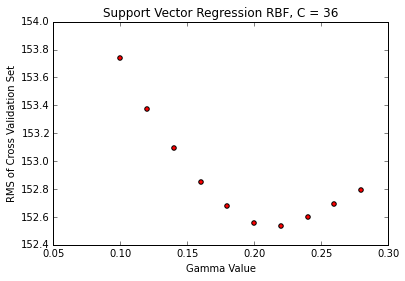
\includegraphics[width=0.45\textwidth]{./images/svmselectgamma.png}

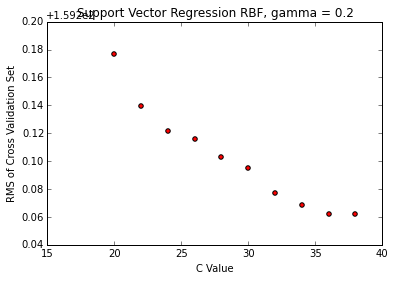
\includegraphics[width=0.45\textwidth]{./images/svmselectc.png}

\end{multicols}

\end{document}
